\begin{enumerate}
	\item 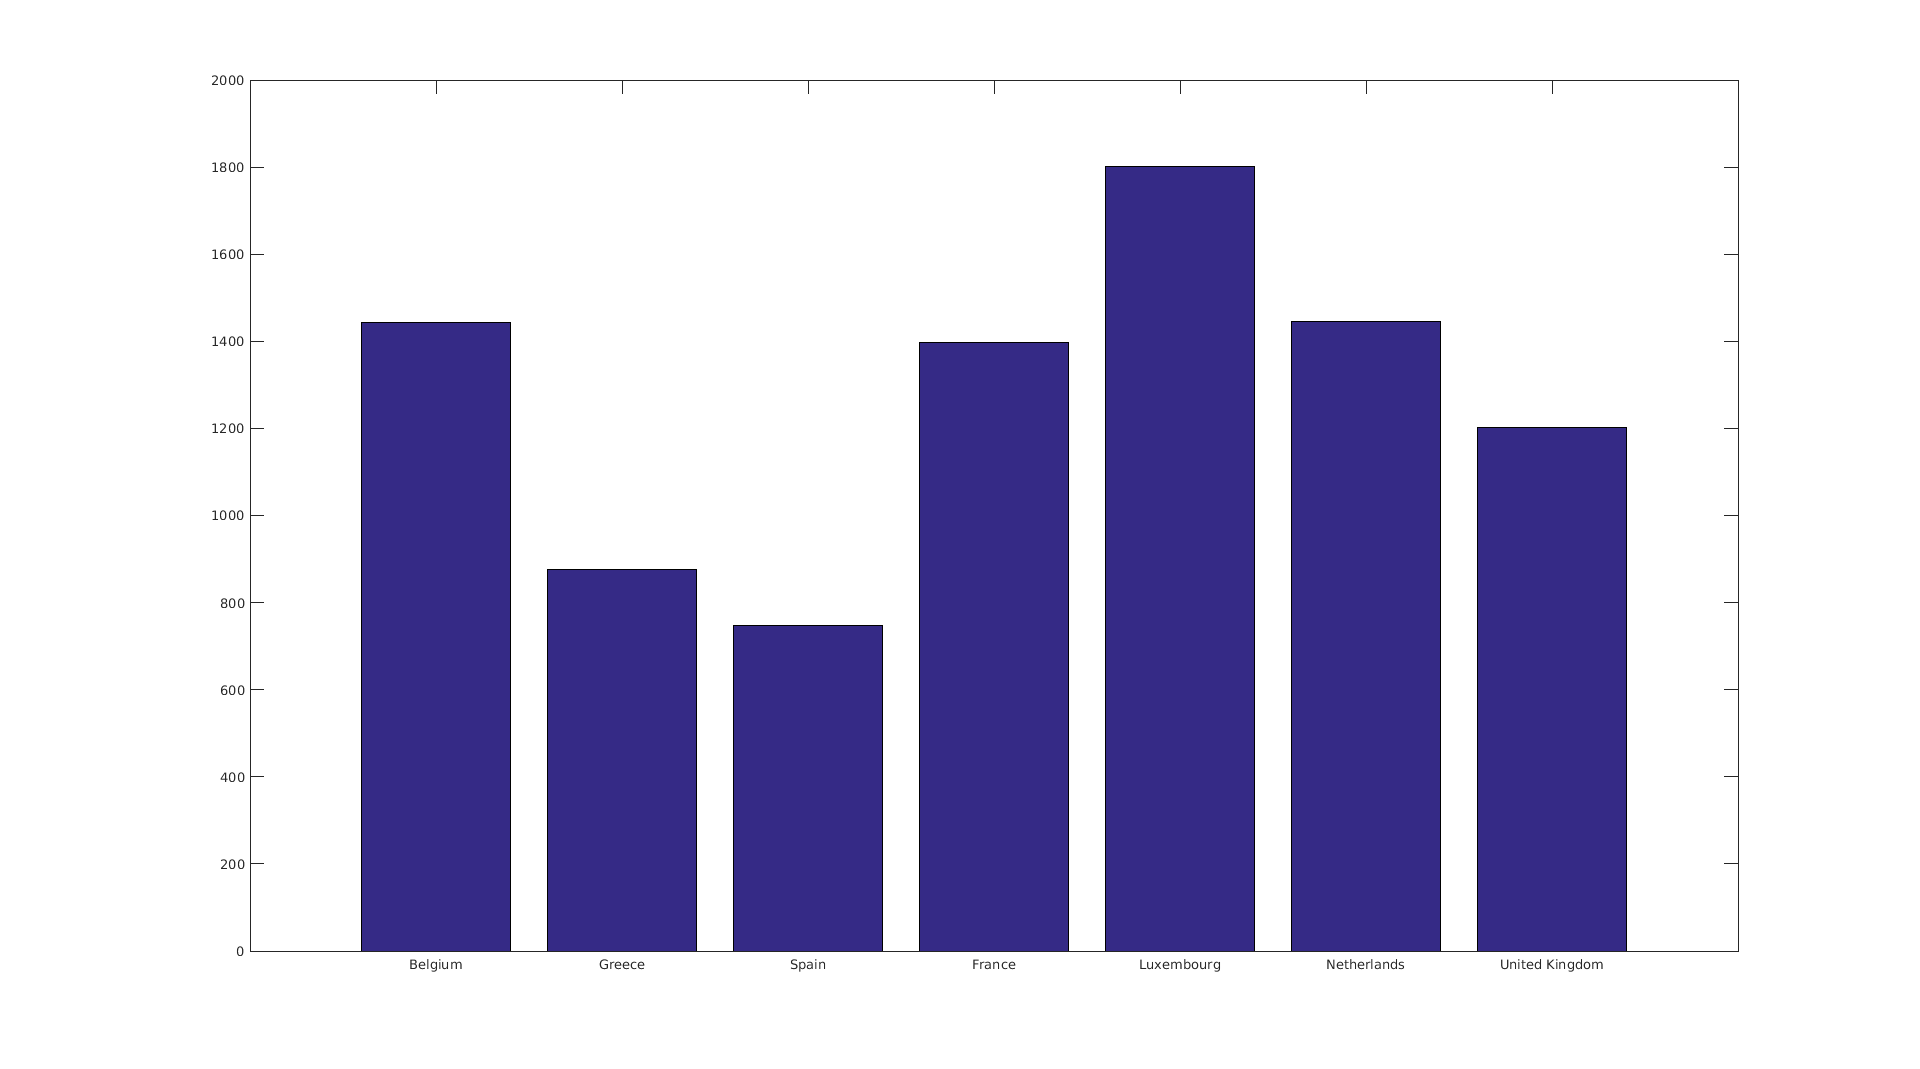
\includegraphics{Graphik/salary_bar}
	\item die Mindestlöhne illustrieren wir mithilfe eines Bar-Charts. Dafür sprechen folgende Punkte:
	\begin{itemize}
		\item es werden nur wenige verglichen
		\item die Werte sind ähnlich
		\item es besteht ein Interesse an dem direkten Vergleich der Werte
	\end{itemize}
	\item 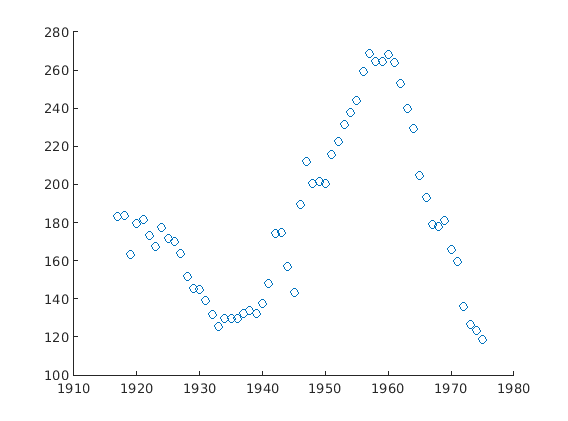
\includegraphics{Graphik/birthrates_scatter.png}
	\item die Geburtsrate stellen wir als Scatter-Plot da. Dafür sprechen folgende Punkte:
	\begin{itemize}
		\item die Daten sind als Tupel mit Zeitpunkt verfügbar
		\item es besteht ein Interesse an der Entwicklung
		\item die Datensätze sind standatisiert
	\end{itemize}
	\item 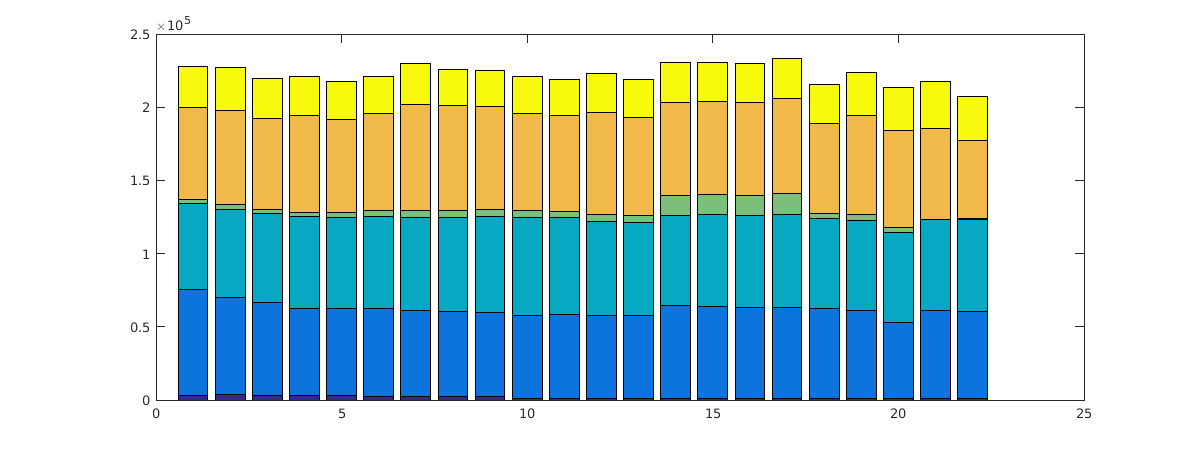
\includegraphics{Graphik/energy_bar}
	\item Die Energieverbrauchsstatistik geben wir als Bar-Chart an
	\begin{itemize}
		\item die 6 Spalten einer Zeile werden immer für eine Balken benutzt und farbig getrennt
		\item jeder Balken (jede Datenzeile) steht für ein Jahr
		\item dadurch lässt sich die Verteilung mehrer Jahre gut vergleichen
	\end{itemize}
	\item 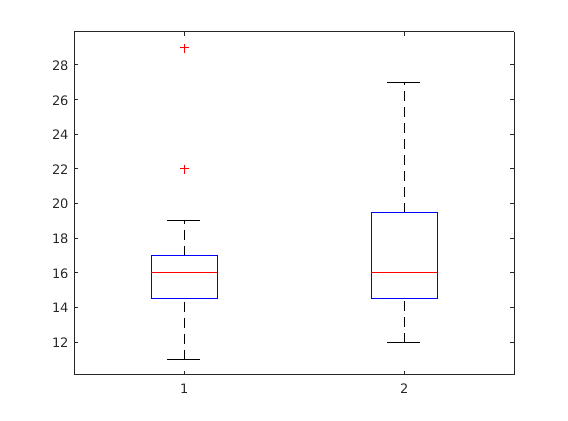
\includegraphics{Graphik/stroop_box}
	\item Für die Visualizierung des Stroop nehmen Boxplots
	\begin{itemize}
		\item zwei Datenreihen, die miteinander verglichen werden
		\item gleiches Experiment
		\item mehrere Ergebnisse
	\end{itemize}
	\item Das Klima wird als timeseries dargestellt
	\item 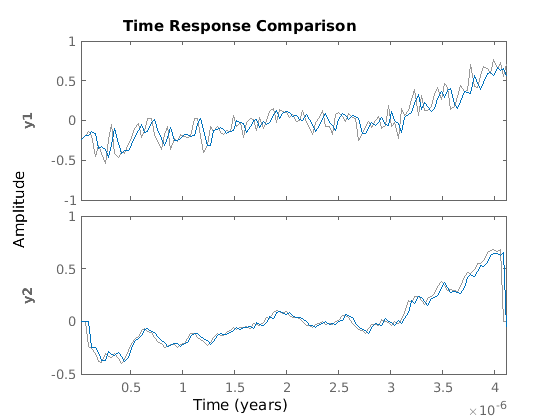
\includegraphics{Graphik/climate_timeseries}
\end{enumerate}
